\documentclass[11pt]{article}
\usepackage{icmlko}
\begin{document}

\title{이득이 는 게 아니라 바닥이 꺼진 것이었다}
\author{월드모델 실험실}
\date{노트 437 · 2026년 8월 6일}
\maketitle

\begin{abstract}
노트 435가 LODO 도메인의 예측 축을 공유 다섯으로 가리면 grp 이득이
$-0.0004 \to +0.0152$ 로 커지는 것을 보이고 ``축의 개수가 절반을 설명한다''고
적었다. 노트 436이 그 예보 쪽을 닫으면서도 \emph{가림은 설계 손잡이로 살아
있다}고 남겨 뒀다. \textbf{그 남은 줄을 갈랐다.}

\begin{center}
\begin{tabular}{lr}
\hline
가림이 \textbf{grp 팔}에 준 변화 & $-0.0261$ \ (음수 $7/11$) \\
가림이 \textbf{무표지 팔}에 준 변화 & $-0.0418$ \ (음수 $6/11$) \\
\hline
이득 변화 & $+0.0157 = -0.0261 - (-0.0418)$ \\
\hline
\end{tabular}
\end{center}

\textbf{두 팔이 다 떨어진다.} 이득이 는 것은 무표지 팔이 더 빨리 떨어져서다
--- \textbf{이득 증가의 $62\%$ 가 바닥이 꺼진 몫}이다. 아이돌은 전부 그렇다:
grp 팔이 $+0.0629 \to +0.0601$ 로 평평한데 무표지 팔이
$+0.1550 \to \mathbf{-0.0625}$ 로 무너져 ``이득''이 $+0.2147$ 로 찍힌다.

\textbf{그러므로 가림은 설계 손잡이가 아니다.} 절대 성적을 내주고 상대 격차를
사는 짓이다.
\end{abstract}

\section{그리고 기계가 다르다}

더 중요한 것이 있다. 가림 실험이 \textbf{집 밖 둘에서 일어나는 일을 재현하지
못한다.}

\begin{center}
\begin{tabular}{lrr}
\hline
 & 무표지 & grp \\
\hline
\textbf{KR 만화} (원래 축 5) & $-0.0822$ & $\mathbf{+0.2128}$ \\
아이돌 (가려서 축 3) & $+0.1550 \to -0.0625$ & $+0.0629 \to +0.0601$ \\
\hline
\end{tabular}
\end{center}

KR 만화는 두 팔이 \textbf{똑같이 축 다섯}인데 grp 가 $-0.08$ 에서 $+0.21$ 로
\textbf{들어올린다}. 가린 아이돌은 grp 팔이 제자리이고 무표지 팔만 꺼진다 ---
\textbf{덜 떨어질 뿐 안 올라간다.}

\textbf{들어올림과 덜 떨어짐은 다른 기계다.} 그러므로 노트 435가 축 개수로
집 밖 둘을 설명했다고 한 것을 \textbf{물린다.} 산수는 맞았고 뜻이 틀렸다.

\section{다시 아무것도 모른다}

집 밖 둘이 유난한 까닭으로 지금까지 죽은 것:

\begin{center}
\begin{tabular}{ll}
\hline
거리 & $\rho = -0.203$, 게다가 집 밖이 더 가깝다 (노트 435) \\
축 개수 --- 예보 & $\rho = -0.451$, 집안만 $-0.248$ (노트 436) \\
축 개수 --- 기계 & 가림은 들어올리지 않고 바닥을 꺼뜨린다 (여기) \\
\hline
\end{tabular}
\end{center}

\textbf{셋 다 죽었다.} 남는 후보는 라벨 계기 · 수집 절차 · 언어처럼 지금
자료로 못 가르는 것들이고, 그것을 가르려면 \textbf{축이 다섯이 아닌 집 밖
도메인}이 있어야 한다 --- 노트 435·436이 이미 적어 둔 그 하나다.

\section{남은 것}

\begin{tabular}{lp{7.0cm}}
\hline
집 밖 셋째 짝 & 세 노트가 연달아 같은 처방에 이른다. 이제 이것 말고 할 것이
없다 \\
아이돌의 무표지 붕괴 & 축을 셋으로 줄이면 $+0.155 \to -0.063$ 이다. 표지 없이
축 셋이면 \textbf{거꾸로 줄을 세운다} --- 노트 398의 KR 만화와 같은 자리 \\
가림 & 설계 손잡이 아님. \textbf{닫는다} \\
\hline
\end{tabular}

\begin{figure}[h]
\centering
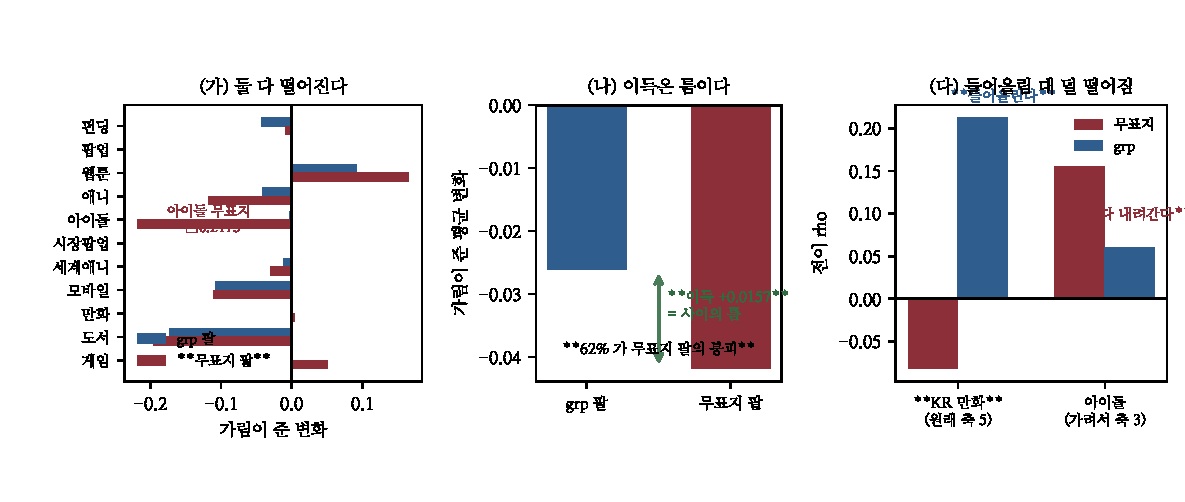
\includegraphics[width=\textwidth]{figs/fig437.pdf}
\caption{(가) 가리면 두 팔이 다 떨어진다. (나) 이득은 두 낙폭 사이의 틈이고
$62\%$ 가 무표지 팔의 붕괴다. (다) KR 만화는 들어올리고 가린 아이돌은 덜
떨어질 뿐이다.}
\end{figure}

\end{document}
